\documentclass[12pt]{article}
\usepackage{graphicx}
\usepackage{minted}
\usepackage{multicol}
\usepackage{subcaption}
\usepackage[english]{babel}
\usepackage{placeins}

\title{Modular Exponentiation and Binary Arithmetic in Python.}
\author{Md Tajim An Noor}
\date{}
\begin{document}
\vspace*{\fill}
\begin{center}

    \emph{Heaven's Light is Our Guide} \\
    \textbf{Rajshahi Universiy of Engineering and Technology} \\

    \begin{figure}[H]
        \centering
        
\includegraphics[scale=.34]{images/RUET_logo.png}
        \label{fig:ruet_logo}
    \end{figure}
    \vspace{5mm}

    \textbf{Course Code}\\
    ECE 2214\\
    \vspace{3mm}
    \textbf{Course Title}\\
    Numerical Methods and Discrete Mathematics Sessional

    \vspace{5mm}
    \textbf{Experiment Date:} October 14, 2023,\\
    \textbf{Submission Date:} {November 4, 2023}\\

    \vspace{5mm}
    \textbf{Lab Report 6:} Finding Chinese remainder theorem \& Carmichael number using python

    \vspace{15mm}

    \begin{tabular}{c|c}
        \textbf{Submitted to} & \textbf{Submitted by} \\
        Md. Nahiduzzaman      & Md. Tajim An Noor     \\
        Lecturer              & Roll: 2010025         \\
        Dept of ECE, Ruet     &                       \\
    \end{tabular}

\end{center}
\vspace*{\fill}

\pagebreak

\tableofcontents

\maketitle
\section{Introduction}


\subsection{Modular Exponentiation}
Modular arithmetic is the branch of arithmetic mathematics related with the “mod” functionality. Basically, modular arithmetic is related with computation of “mod” of expressions. Expressions may have digits and computational symbols of addition, subtraction, multiplication, division or any other. Here we will discuss briefly about all modular arithmetic operations.\\
The result of ($a \wedge b \:mod\: m$) is the modular exponentiation.
\cite{gfgMod}

\subsection{Binary Arithmetic}
Binary number system uses only two digits, $0$ \& $1$. The basic arithmetic operations like addition and subtraction are known as binary arithmetic. Binary arithmetic starts from the least significant bit of a binary number and gradually goes towards the most significant bit.

\section{Tools Used}
\begin{itemize}
    \item Python
    \item VS Code - for running python code
    \item MacTeX -\LaTeX  compiler
    \item VS Code with \LaTeX workshop extension as a text editor
\end{itemize}

\section{Process}

\subsection{Code:}
\subsubsection{Modular Exponentiation}
\inputminted[breaklines,linenos]{python3}{codes/amodularExpo.py}

\vspace{13mm}

\subsubsection{Binary Arithmetic}
\inputminted[breaklines,linenos]{python3}{codes/bbinaryAddSub.py}

\vspace{13mm}

\subsubsection{Integrated}
\inputminted[breaklines,linenos]{python3}{codes/cintegrated.py}

\vspace{20mm}
\subsection{Output}
\begin{figure}[H]
    \begin{subfigure}{.5\textwidth}
        \centering
        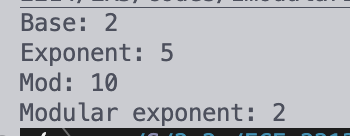
\includegraphics[width=.8\linewidth, height = .73in]{images/output/expo1.png}
        \caption*{}
        \label{fig:expo1}
    \end{subfigure}
    \begin{subfigure}{.5\textwidth}
        \centering
        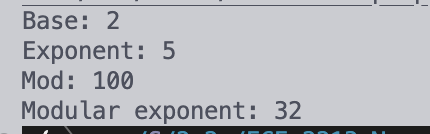
\includegraphics[width=.8\linewidth]{images/output/expo2.png}
        \caption*{}
        \label{fig:expo2}
    \end{subfigure}
    \begin{subfigure}{.5\textwidth}
        \centering
        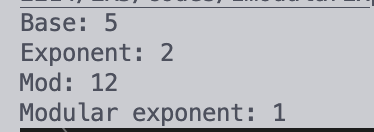
\includegraphics[width=.8\linewidth]{images/output/expo3.png}
        \caption*{}
        \label{fig:expo3}
    \end{subfigure}
    \begin{subfigure}{.5\textwidth}
        \centering
        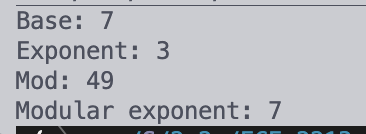
\includegraphics[width=.8\linewidth]{images/output/expo4.png}
        \caption*{}
        \label{fig:expo4}
    \end{subfigure}
    \caption{Outputs for Modular Exponentiation}
    \label{fig:expo}
\end{figure}
\begin{figure}[H]
    \begin{subfigure}{.5\textwidth}
        \centering
        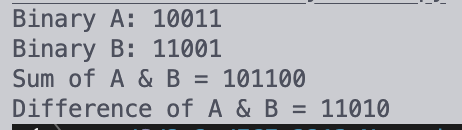
\includegraphics[width=.8\linewidth]{images/output/bin1.png}
        \caption*{}
        \label{fig:bin1}
    \end{subfigure}
    \begin{subfigure}{.5\textwidth}
        \centering
        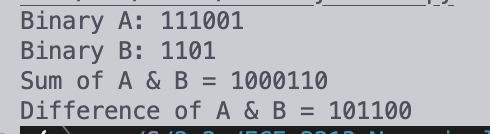
\includegraphics[width=.8\linewidth]{images/output/bin2.png}
        \caption*{}
        \label{fig:bin2}
    \end{subfigure}
    \newline
    \begin{subfigure}{.5\textwidth}
        \centering
        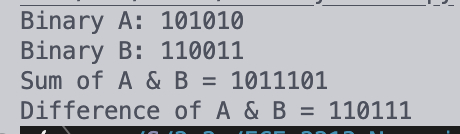
\includegraphics[width=.8\linewidth]{images/output/bin3.png}
        \caption*{}
        \label{fig:bin3}
    \end{subfigure}
    \begin{subfigure}{.5\textwidth}
        \centering
        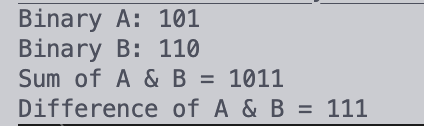
\includegraphics[width=.8\linewidth]{images/output/bin4.png}
        \caption*{}
        \label{fig:bin4}
    \end{subfigure}
    \caption{Outputs for Contraposition}
    \label{fig:bin}
\end{figure}

\begin{figure}[H]
    \begin{subfigure}{.5\textwidth}
        \centering
        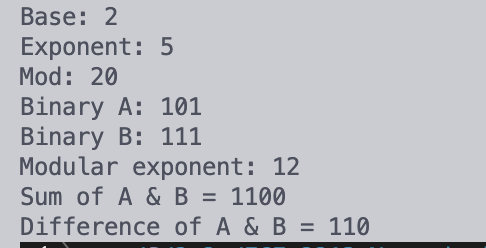
\includegraphics[width=.8\linewidth]{images/output/int1.png}
        \caption*{}
        \label{fig:int1}
    \end{subfigure}
    \begin{subfigure}{.5\textwidth}
        \centering
        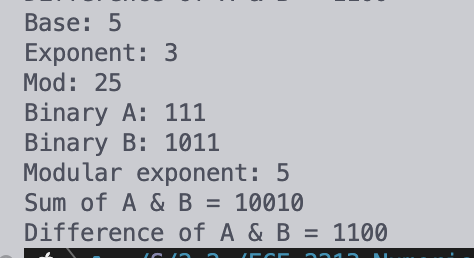
\includegraphics[width=.8\linewidth, height=1.1in]{images/output/int2.png}
        \caption*{}
        \label{fig:int2}
    \end{subfigure}
    \begin{subfigure}{.5\textwidth}
        \centering
        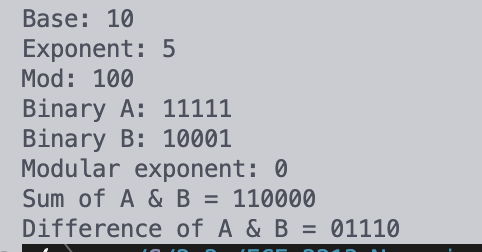
\includegraphics[width=.8\linewidth,]{images/output/int3.png}
        \caption*{}
        \label{fig:int3}
    \end{subfigure}
    \begin{subfigure}{.5\textwidth}
        \centering
        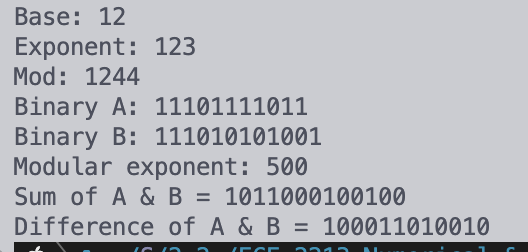
\includegraphics[width=.8\linewidth]{images/output/int4.png}
        \caption*{}
        \label{fig:int4}
    \end{subfigure}
    \caption{Outputs for Logical Equivalence}
    \label{fig:int}
\end{figure}

\section{Discussion}
In the first code, the modular exponentiation, 3 inputs are taken: base, exponent \& mod. The base is the number that exponent will be done upon, exponent is the power for the base. Using an algorithm, getting way too large number can be avoided. The result is the base to the power of exponent modded by mod.\\
For the binary arithmetic operations; when adding two binary number, the iteration is done from LSB to MSB. If there is a carry, its calculated accordingly.\\
For the subtracting operation the 2nd number is converted to its 2's compliment equivalent. And then it was added using the adding function. Then after the addition was done, it was checked if there was any carry bit. If there were any, the result was converted to its equivalent 2's compliment and shown.

\bibliographystyle{IEEEtran}
\bibliography{ref}

\end{document}